\subsection{Max Pooling Layer}

After the convolutional layer a pooling layer is placed. This reduces the dimensionality of the data as well as introduces local non-linearity to the network, enabling it to achieve better function approximation. In our case the layer performs a max operation among a $2 \times 2$ image patch. This means that a 2-by-2 image patch is mapped to 1 output pixel and it's value is equivalent to the maximum value of the input image patch.
Because of the processing of the convolutional layer (see Figure~\ref{fig:hw-conv-operation}) a whole input image input row must be buffered before any processing can happen. Because the pooling layer requires a $2$-by-$2$ input window it is limited by the output of the convolutional layer. To increase throughput the convolutional layer could be parallelized by doing two convolutions at once at the cost of increased area size. Alternatively the pooling operation can be serialized by only operating on half the output channels of the convolutional layer at a time.

\begin{figure}[hb]
	\centering
	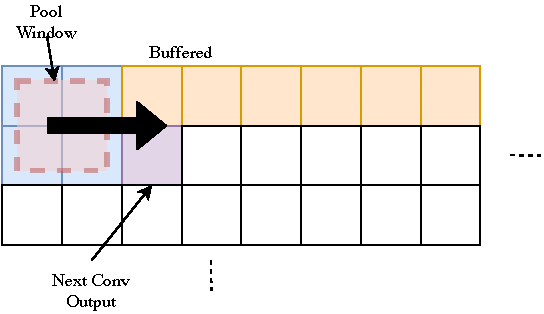
\includegraphics[width=0.6\textwidth]{img/pool.pdf}
	\caption[Pooling Operation]{Pooling Operation. The pool window (red-dashed-square) applied to current image patch (blue) and shifted over the input data. The first input row needs to be buffered (orange) before processing can happen. Depth channels omitted for illustration purposes.}
	\label{fig:hw-conv-operation}
\end{figure}



\begin{table}[hb]
	\centering
	\begin{tabular}{lcc}
		\toprule
		Parameter & VHDL Datatype & Type \\
		\midrule
		 BIT\_WIDTH\_IN & integer & Generic	 	\\
		 BIT\_WIDTH\_OUT & integer & Generic 	\\
		 INPUT\_CHANNELS & integer & Generic 	\\
 	 	 OUTPUT\_CHANNELS & integer & Generic 	\\
 	 	 \midrule
 	 	 valid\_i & \stdlogic & input \\
 	 	 data\_i & \stdlogic[INPUT\_CHANNELS][DATA\_WIDTH] & input \\
 	 	 \midrule
 	 	 valid\_o & \stdlogic & output \\
 	 	 data\_o & \stdlogic[INPUT\_CHANNELS][DATA\_WIDTH] & output \\
   		\bottomrule
	\end{tabular}
	\caption{}
	\label{tab:hw-pool-layer-parameter}
\end{table}
